\thispagestyle{quantoannone}
\pagestyle{quantoan}
\everymath{\color{quantoan}}
\graphicspath{{../quantoan/pic/}}
%\blfootnote{\color{quantoan}\color{quantoan}$^*$Nguồn Math. Intellegencer, Số $41$.}
\begingroup
\AddToShipoutPicture*{\put(0,616){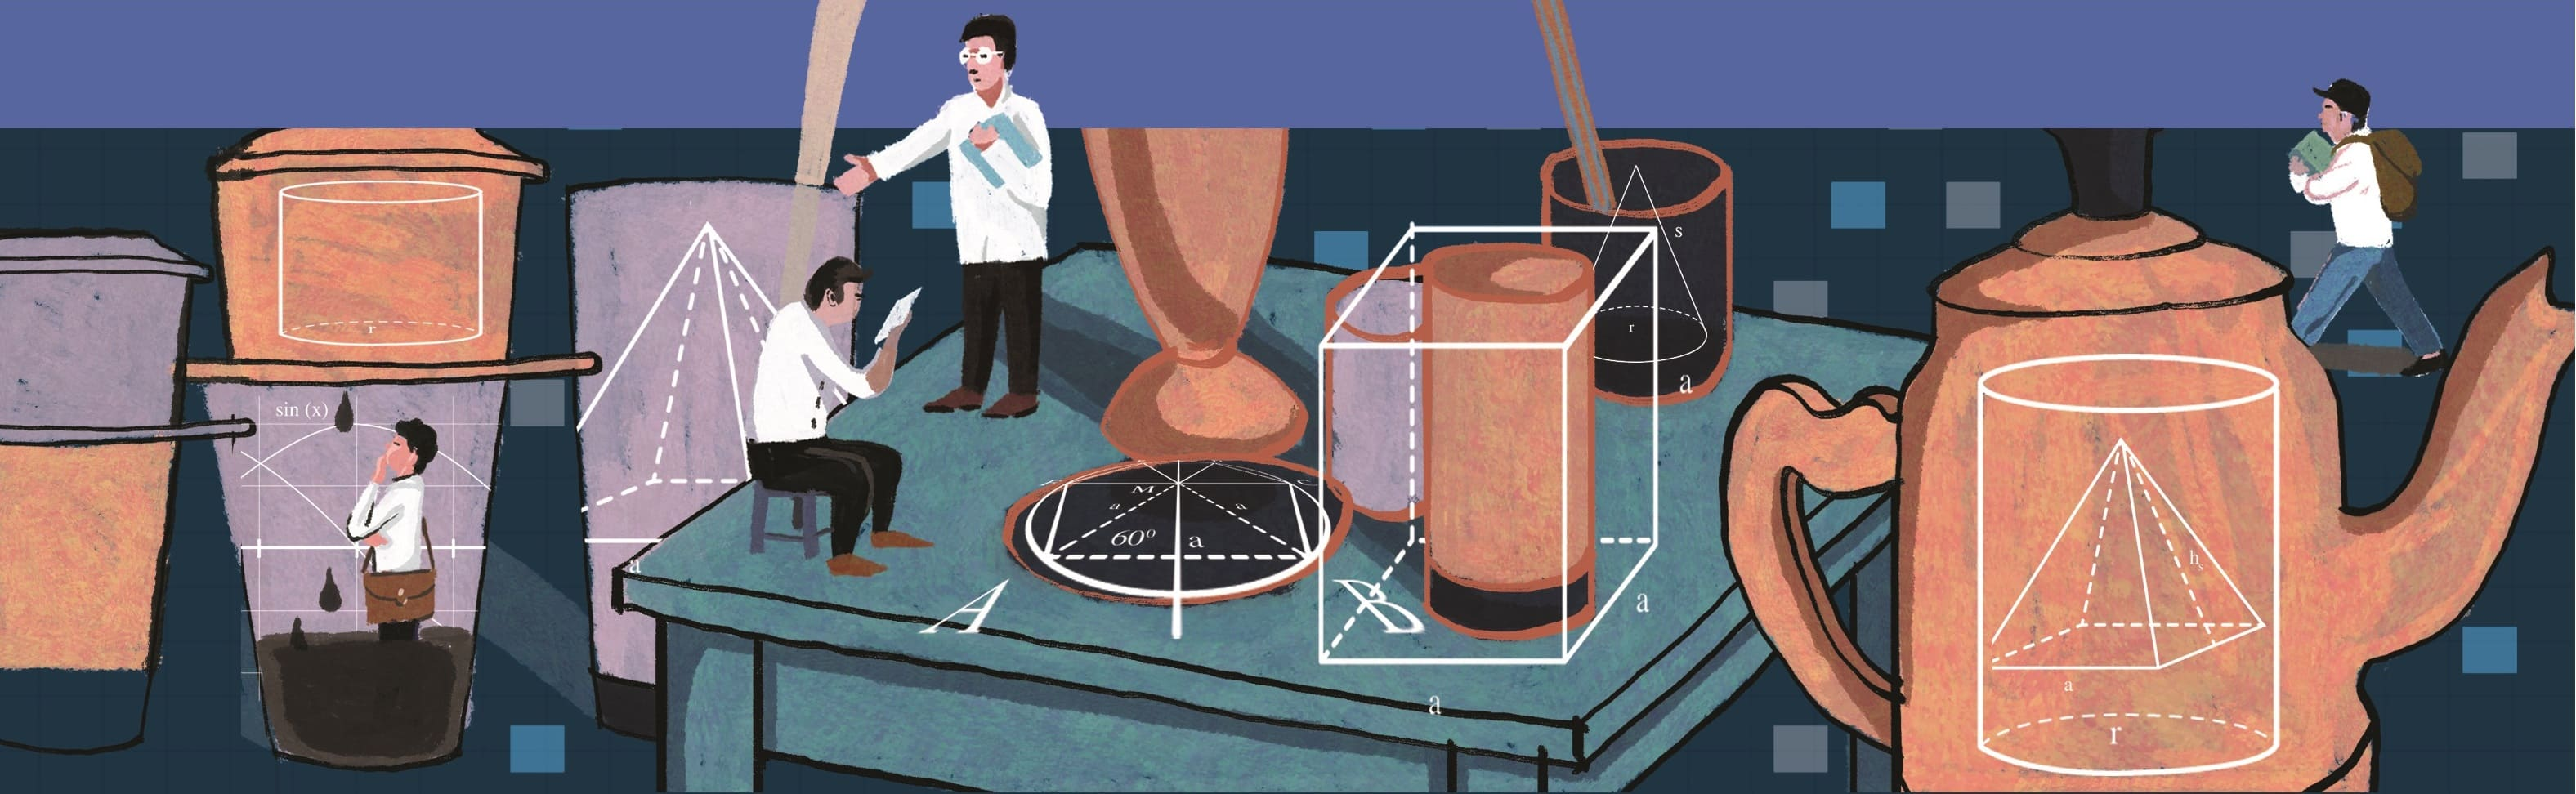
\includegraphics[width=19.3cm]{../bannerquantoan}}}
\AddToShipoutPicture*{\put(120,552){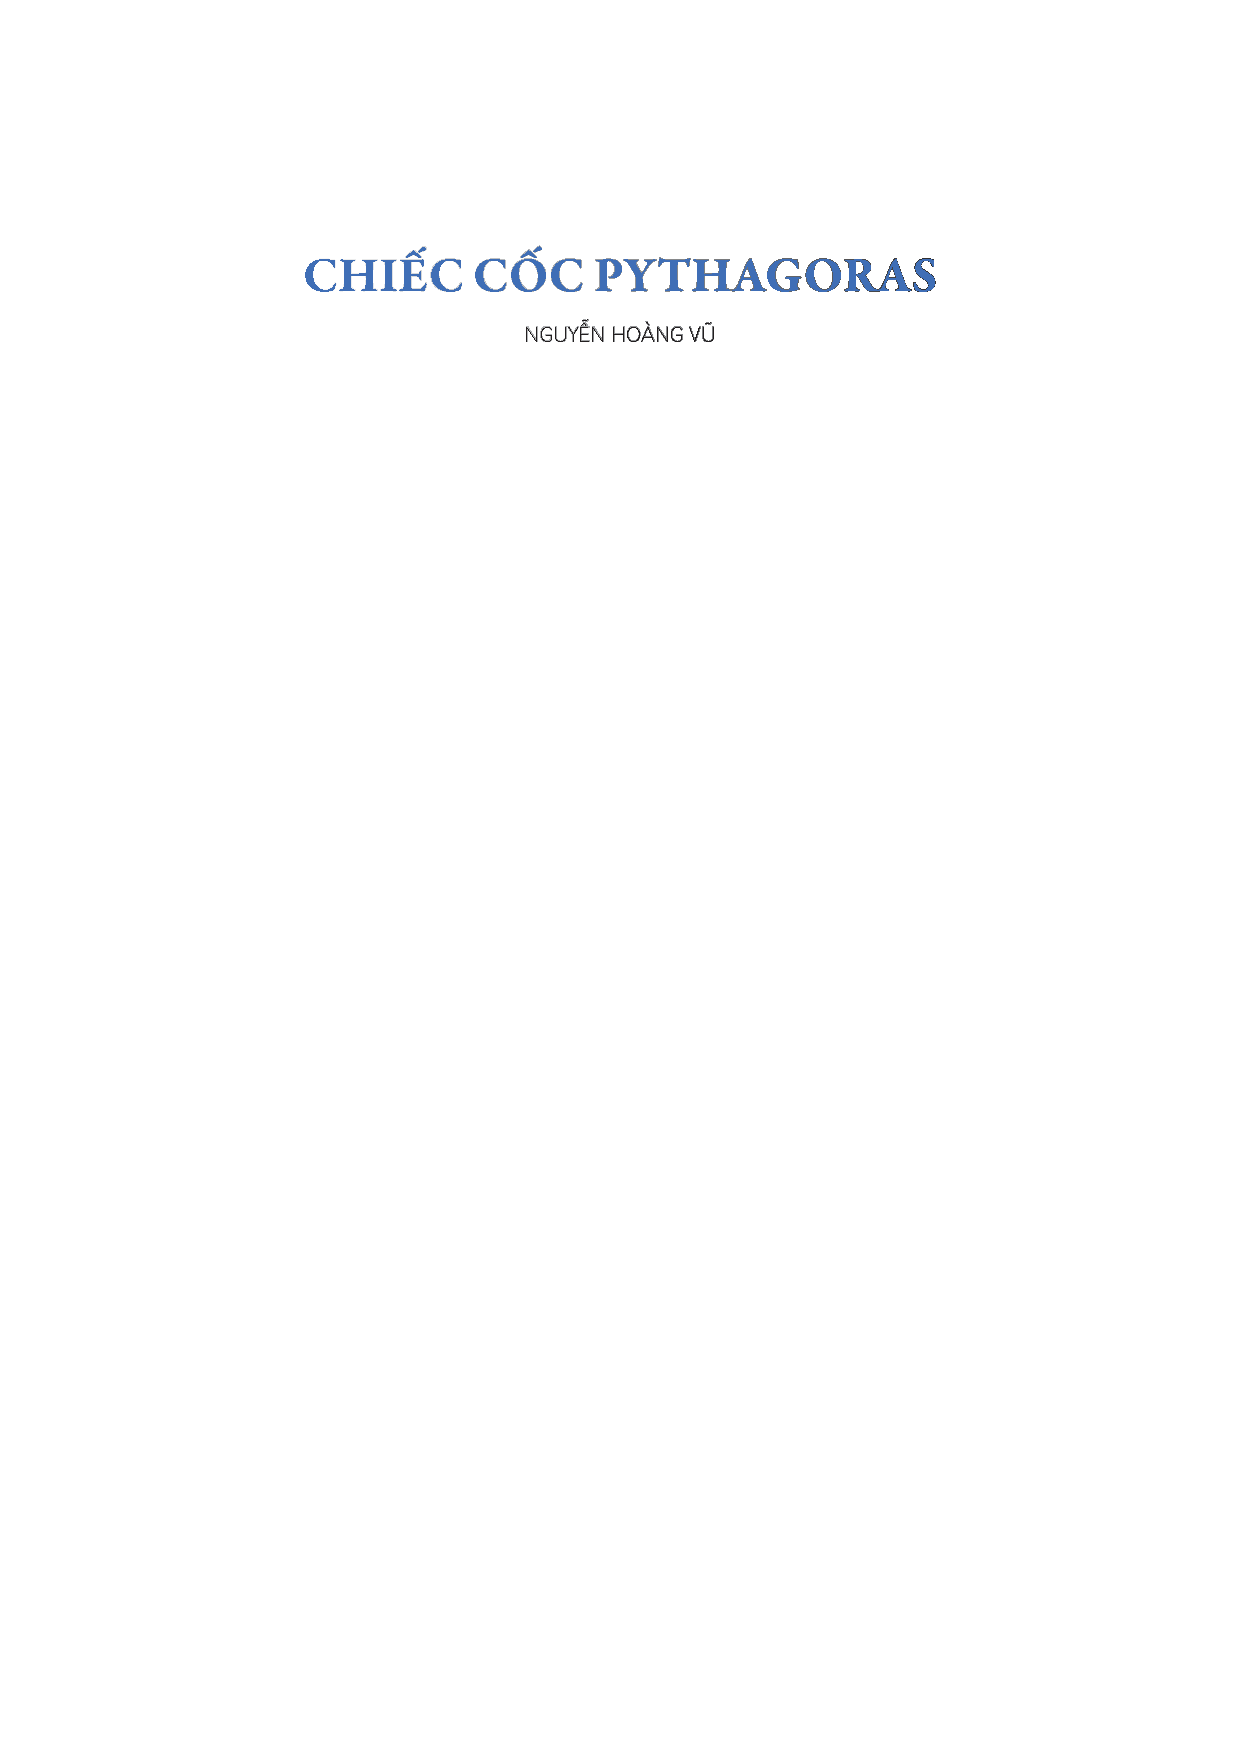
\includegraphics[scale=1]{../tieude.pdf}}}
\centering
\endgroup
\vspace*{155pt}

\begin{multicols}{2}
	Ta hãy kết thúc bài viết bằng một hiện tượng có phần kỳ lạ liên quan đến bình thông nhau. 
	\begin{figure}[H]
		\vspace*{-5pt}
		\centering
		\captionsetup{labelformat= empty, justification=centering}
		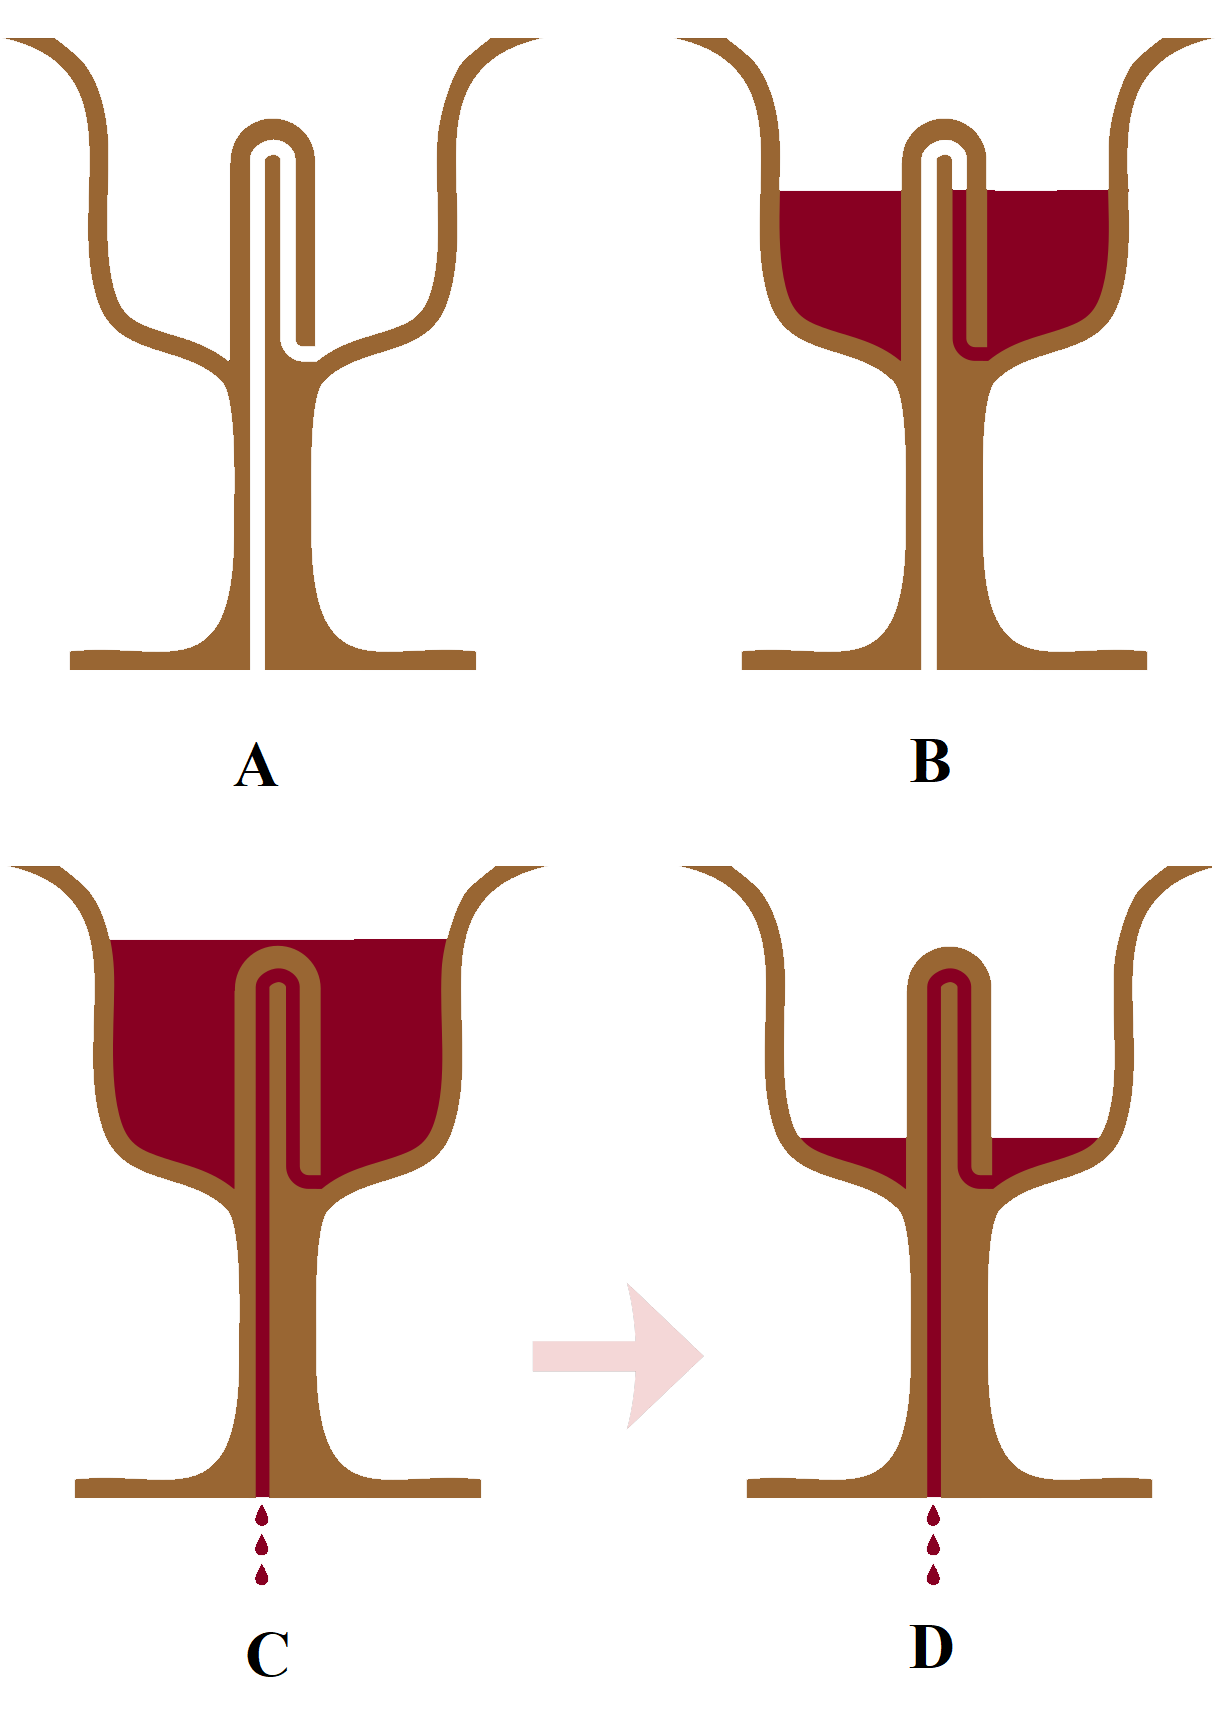
\includegraphics[width= 1\linewidth]{1}
		\caption{\small\textit{\color{quantoan}Hình $1$. Chiếc cốc của Pythagoras. Khi rót đầy chất lỏng vượt ngưỡng, toàn bộ chất lỏng trong cốc sẽ bị chảy ra ngoài}}
		\vspace*{-10pt}
	\end{figure}
	Người ta kể lại rằng nhà toán học Pythagoras đã thiết kế một loại cốc đặc biệt dành cho các học trò của mình (Hình $1$). Ở phần giữa của nó có một lỗ thông xuống đáy được che lại bởi một cấu trúc tạo thành bình thông nhau. Khi đổ dần rượu vào cốc, mực rượu sẽ dâng lên ở trong cốc cũng như nhánh thông với nó (Hình $1$B). Đến khi mực rượu vượt ngưỡng chứa của nhánh này, nó bắt đầu sẽ bị chảy ra ngoài (Hình $1$C). Nhưng thay vì chỉ rút xuống mức tới hạn trước khi rượu bắt đầu chảy ra, toàn bộ chất lỏng trong cốc lại vẫn tiếp tục tạo thành dòng chảy ra ngoài cho đến khi chảy hết rượu. Những kẻ tham lam sẽ không còn lại gì cả!
	\vskip 0.1cm
	Đây là một bài học của Pythagoras cho các học trò của mình về việc phải có chừng mực trong cuộc sống, không được thái quá. Vậy còn bài học về vật lý ở đây là gì? Tại sao rượu lại có thể tiếp tục chảy ngược ra ngoài dù mực rượu trong phần ống cao hơn trong cốc? Những gì ta đã biết về bình thông nhau có bị vi phạm?
	\vskip 0.1cm
	Thực chất của hiện tượng xảy ra trong chiếc cốc của Pythagoras giống với quy trình hoạt động của ống siphon (Hình $2$). Ống này có dạng ống chữ U ngược với hai đầu đặt ở hai khối chất lỏng khác nhau, một đầu cao hơn đầu còn lại. Chất lỏng trong ống siphon có thể chảy từ khối chất lỏng cao ngược lên đỉnh chữ U rồi chảy xuống khối chất lỏng ở dưới. Để bắt đầu dòng chảy, người ta cần hút không khí ra khỏi đầu dưới của ống để tạo sự chênh lệch với áp suất khí quyển ở đầu còn lại. Hai mô hình được đưa ra để giải thích hiện tượng này. Trong mô hình thứ nhất, khi chất lỏng chảy vượt qua đỉnh của chữ U ngược, nó tạo ra một vùng áp suất thấp nên áp suất khí quyển từ đầu đường ống sẽ tiếp tục đẩy chất lỏng đi. Mô hình thứ hai dựa trên lực liên kết phân tử, trong đó sự kết dính giữa các khối nước sẽ kéo chúng theo nhau tạo thành dòng chảy. Việc mô hình nào là chính xác vẫn còn là một vấn đề đang được khoa học nghiên cứu.
	\begin{figure}[H]
		\vspace*{-5pt}
		\centering
		\captionsetup{labelformat= empty, justification=centering}
		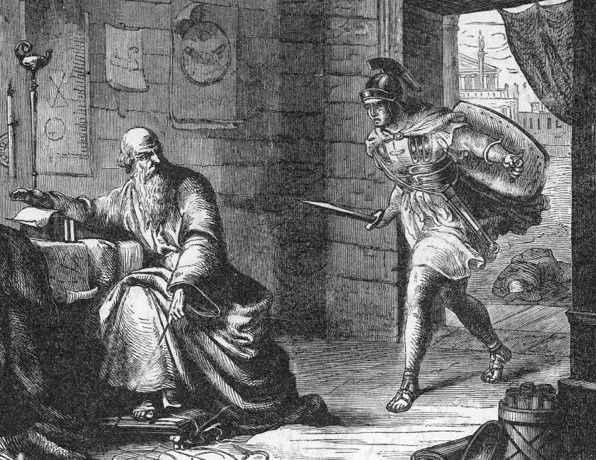
\includegraphics[width= 1\linewidth]{2}
		\caption{\small\textit{\color{quantoan}Hình $2$. Ống siphon có thể tạo dòng chảy đỉ lên ngược với chiều của trọng lực nếu hai đầu của chữ U ngược có độ cao khác nhau.}}
		\vspace*{-10pt}
	\end{figure}
	Nếu nhìn lại vào cấu tạo của chiếc cốc Pythagoras, ta có thể thấy ngay một đoạn chữ U ngược tương tự như ống siphon với một đầu nối với lòng cốc và đầu còn lại nối với chân cốc. Trong thực tế, ống siphon được sử dụng thường xuyên trong đời sống để tháo nước khỏi các bình chứa, lấy bia ra khỏi thùng bia, rút nước khỏi các mái nhà có diện tích lớn, hay trong khay đựng bột giặt của các máy giặt, ...  Một số nghiên cứu khảo cổ cũng cho thấy ống siphon đã được sử dụng từ thời Ai Cập cổ đại trong nhiều công việc như dẫn nước thủy lợi hay chế biến đồ uống. 
	\begin{figure}[H]
		\vspace*{-5pt}
		\centering
		\captionsetup{labelformat= empty, justification=centering}
		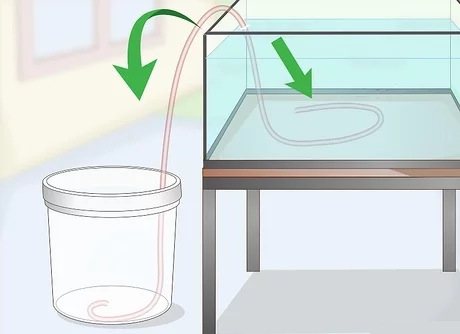
\includegraphics[width= 1\linewidth]{3}
		\caption{\small\textit{\color{quantoan}Hình $3$. Ống siphon dùng để rút nước khỏi bể chứa.}}
		\vspace*{-10pt}
	\end{figure}
\end{multicols}